%%%%%%%%%%%%%%%%%%%%%%%%%%%%%%%%%%%%%%%%%%%%%%%%%%%%%%%%%%%%%%%%%%%%%%%%%%%%%%%%%%%%%%%%%%%%%%%%%%%%%%%%%%%%%%%%%%%%%%%%%%%%%%%%%%%%%%%%%%%%%%%%%%%%%%%%%%%%%%%%%%%
% Written By Michael Brodskiy
% Class: Fundamentals of Electronics
% Professor: I. Salama
%%%%%%%%%%%%%%%%%%%%%%%%%%%%%%%%%%%%%%%%%%%%%%%%%%%%%%%%%%%%%%%%%%%%%%%%%%%%%%%%%%%%%%%%%%%%%%%%%%%%%%%%%%%%%%%%%%%%%%%%%%%%%%%%%%%%%%%%%%%%%%%%%%%%%%%%%%%%%%%%%%%

\include{Includes.tex}

\title{Pre-Lab 5}
\date{November 11, 2024}
\author{Michael Brodskiy\\ \small Professor: M. Onabajo}

\begin{document}

\maketitle

\begin{enumerate}

  \item We may begin by performing a DC analysis of the circuit. As a result, we may see that $I_D$ and $V_{DS}$ need to be calculated. Assuming performance in the saturation region (since this is preferred for amplification), we may write:

    $$I_D=\frac{1}{2}\mu_n\cos\left( \frac{w}{L} \right)\left( V_{GS}-V_{t} \right)^2$$

    We can substitute in known values to obtain:

    $$I_D=\frac{1}{2}\left( .25\cdot10^{-3} \right)\left( 2-1 \right)^2$$
    $$\boxed{I_D=.125[\si{\milli\ampere}]}$$

    From this, we may write:

    $$-V_{DD}+R_DI_D+V_D=0$$
    $$V_D=V_{DD}-R_DI_D$$

    We now substitute known values to get:

    $$V_D=(10)-(10k)(.125m)$$
    $$\boxed{V_D=8.75[\si{\volt}]}$$

    To confirm saturation conditions, we get:

    $$V_{DS}\geq V_{GS}-V_t$$

    $$V_{DS}=V_{DD}-V_{D}$$
    $$V_{DS}=10-8.75$$
    $$\boxed{V_{DS}=1.25[\si{\volt}]}$$

    Since $1.25\geq 1$, we may conclude that we are, as a matter of fact, operating in saturation. We may proceed to calculation of a Th\'evenin equivalent:

    $$V_{th}=V_{DD}\left( \frac{R_{G2}}{R_{G1}+R_{G2}} \right)$$
    $$R_{th}=\left( \frac{R_{G1}R_{G2}}{R_{G1}+R_{G2}} \right)$$
    $$R_{th}=\left( \frac{R_{G1}R_{G2}}{R_{G1}+R_{G2}} \right)$$

    To find the correct values, we use KVL to write:

    $$-V_{DD}+I_DR_D+V_{DS}+V_{S}=0$$

    This lets us find $V_{S}$:

    $$V_{S}=10-8.75-1.25$$
    $$V_{S}=0[\si{\volt}]$$

    Since we know the value of $V_{GS}$, we write:

    $$V_{GS}=V_G-V_S$$
    $$2=V_G-V_S$$

    Thus, we find that $V_G=V_{th}=2[\si{\volt}]$. We may then write:

    $$2=\frac{10R_{G2}}{R_{G1}+R_{G2}}$$
    $$R_{G1}+R_{G2}=5R_{G2}$$
    $$R_{G1}=4R_{G2}$$

    We can take any values for which the above statement is true. As such, let us use:

    $$\boxed{R_{G1}=4[\si{\mega\ohm}]\quad\text{ and }R_{G2}=1[\si{\mega\ohm}]}$$

  \item Read through, no questions \textcolor{green}{\checkmark}

  \item We may combine some CD4007s to obtain (Note A, B, and C are the push-button inputs):

    \begin{figure}[H]
      \centering
      \tikzset{every picture/.style={line width=0.75pt}} %set default line width to 0.75pt        

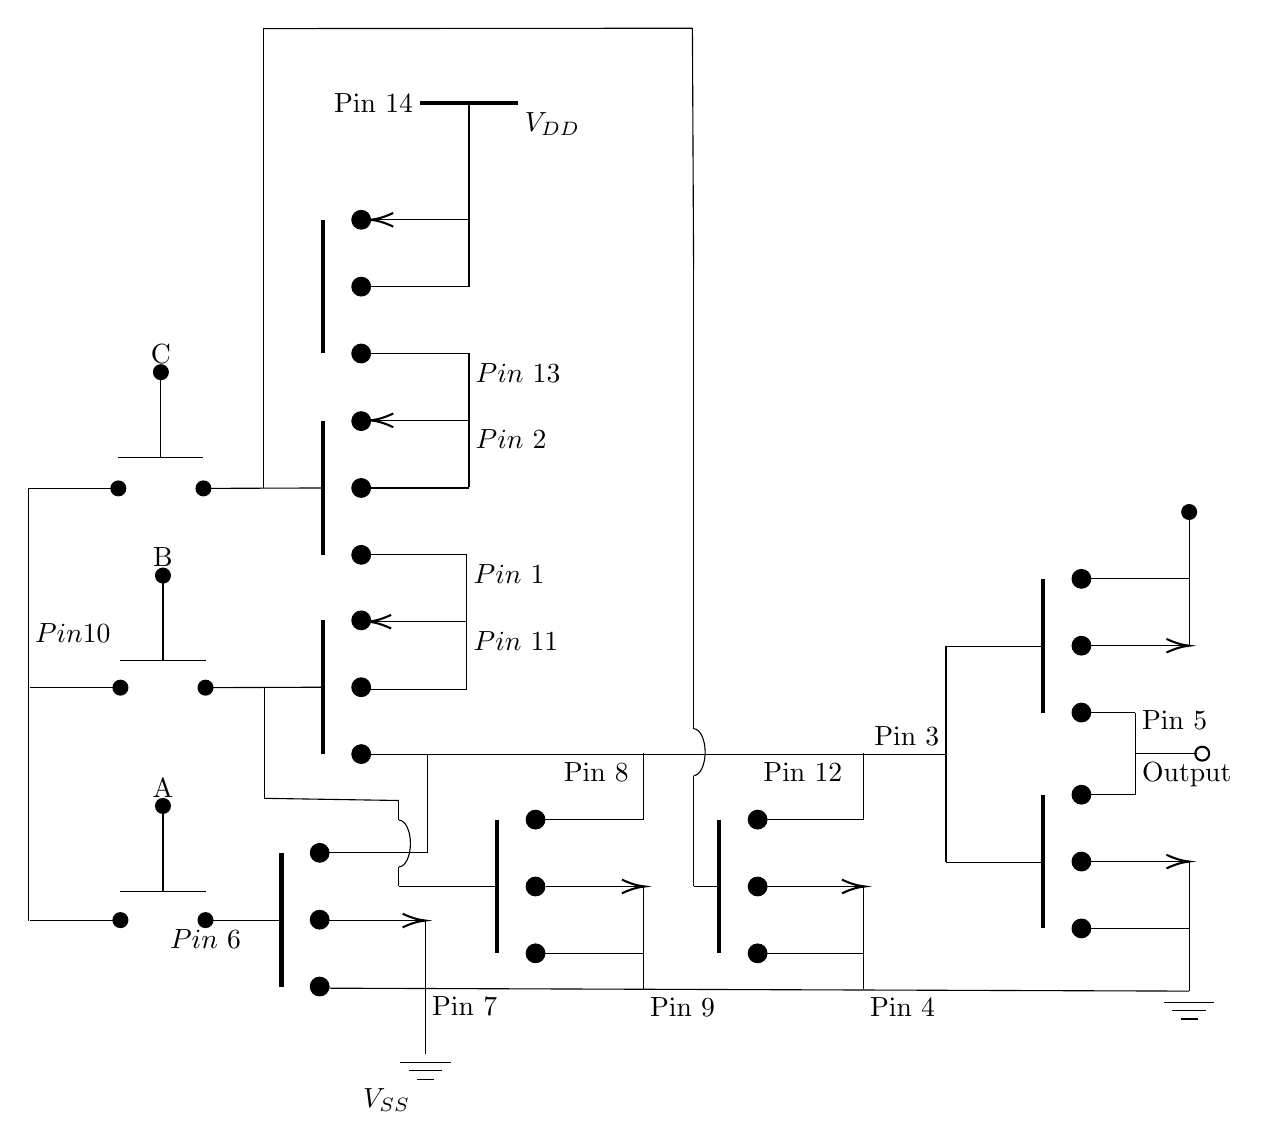
\begin{tikzpicture}[x=0.75pt,y=0.75pt,yscale=-1,xscale=1]
%uncomment if require: \path (0,590); %set diagram left start at 0, and has height of 590

%Straight Lines [id:da881261368948268] 
\draw [line width=1.5]    (176,105.29) -- (176,169.71) ;
%Shape: Circle [id:dp4547836215599118] 
\draw  [fill={rgb, 255:red, 0; green, 0; blue, 0 }  ,fill opacity=1 ] (189.92,105.29) .. controls (189.92,102.8) and (191.94,100.79) .. (194.42,100.79) .. controls (196.91,100.79) and (198.92,102.8) .. (198.92,105.29) .. controls (198.92,107.77) and (196.91,109.79) .. (194.42,109.79) .. controls (191.94,109.79) and (189.92,107.77) .. (189.92,105.29) -- cycle ;
%Shape: Circle [id:dp7535055234156659] 
\draw  [fill={rgb, 255:red, 0; green, 0; blue, 0 }  ,fill opacity=1 ] (189.92,137.5) .. controls (189.92,135.01) and (191.94,133) .. (194.42,133) .. controls (196.91,133) and (198.92,135.01) .. (198.92,137.5) .. controls (198.92,139.99) and (196.91,142) .. (194.42,142) .. controls (191.94,142) and (189.92,139.99) .. (189.92,137.5) -- cycle ;
%Shape: Circle [id:dp2701544083948245] 
\draw  [fill={rgb, 255:red, 0; green, 0; blue, 0 }  ,fill opacity=1 ] (189.92,169.71) .. controls (189.92,167.23) and (191.94,165.21) .. (194.42,165.21) .. controls (196.91,165.21) and (198.92,167.23) .. (198.92,169.71) .. controls (198.92,172.2) and (196.91,174.21) .. (194.42,174.21) .. controls (191.94,174.21) and (189.92,172.2) .. (189.92,169.71) -- cycle ;

%Straight Lines [id:da5228905760160462] 
\draw    (246.34,105.29) -- (200.92,105.29) ;
\draw [shift={(198.92,105.29)}, rotate = 360] [color={rgb, 255:red, 0; green, 0; blue, 0 }  ][line width=0.75]    (10.93,-3.29) .. controls (6.95,-1.4) and (3.31,-0.3) .. (0,0) .. controls (3.31,0.3) and (6.95,1.4) .. (10.93,3.29)   ;
%Straight Lines [id:da4160636329408052] 
\draw    (246.34,48.87) -- (246.34,137.5) ;
%Straight Lines [id:da9824219257539123] 
\draw [line width=1.5]    (270.05,48.87) -- (222.63,48.87) ;
%Straight Lines [id:da788560025252111] 
\draw    (246.34,137.5) -- (198.92,137.5) ;
%Straight Lines [id:da6902776170249463] 
\draw [line width=1.5]    (176,202.29) -- (176,266.71) ;
%Shape: Circle [id:dp9379739424065744] 
\draw  [fill={rgb, 255:red, 0; green, 0; blue, 0 }  ,fill opacity=1 ] (189.92,202.29) .. controls (189.92,199.8) and (191.94,197.79) .. (194.42,197.79) .. controls (196.91,197.79) and (198.92,199.8) .. (198.92,202.29) .. controls (198.92,204.77) and (196.91,206.79) .. (194.42,206.79) .. controls (191.94,206.79) and (189.92,204.77) .. (189.92,202.29) -- cycle ;
%Shape: Circle [id:dp5383036634662248] 
\draw  [fill={rgb, 255:red, 0; green, 0; blue, 0 }  ,fill opacity=1 ] (189.92,234.5) .. controls (189.92,232.01) and (191.94,230) .. (194.42,230) .. controls (196.91,230) and (198.92,232.01) .. (198.92,234.5) .. controls (198.92,236.99) and (196.91,239) .. (194.42,239) .. controls (191.94,239) and (189.92,236.99) .. (189.92,234.5) -- cycle ;
%Shape: Circle [id:dp01295226009519057] 
\draw  [fill={rgb, 255:red, 0; green, 0; blue, 0 }  ,fill opacity=1 ] (189.92,266.71) .. controls (189.92,264.23) and (191.94,262.21) .. (194.42,262.21) .. controls (196.91,262.21) and (198.92,264.23) .. (198.92,266.71) .. controls (198.92,269.2) and (196.91,271.21) .. (194.42,271.21) .. controls (191.94,271.21) and (189.92,269.2) .. (189.92,266.71) -- cycle ;

%Straight Lines [id:da7380183153774791] 
\draw    (246.34,169.71) -- (198.92,169.71) ;
%Straight Lines [id:da21903553431005474] 
\draw    (246.34,201.92) -- (200.92,201.92) ;
\draw [shift={(198.92,201.92)}, rotate = 360] [color={rgb, 255:red, 0; green, 0; blue, 0 }  ][line width=0.75]    (10.93,-3.29) .. controls (6.95,-1.4) and (3.31,-0.3) .. (0,0) .. controls (3.31,0.3) and (6.95,1.4) .. (10.93,3.29)   ;
%Straight Lines [id:da5695558202993837] 
\draw    (246.34,201.92) -- (246.34,169.71) ;
%Straight Lines [id:da5976800135416879] 
\draw    (246.34,234.5) -- (198.92,234.5) ;
%Straight Lines [id:da5143206271139323] 
\draw    (246.34,234.13) -- (246.34,201.92) ;

%Straight Lines [id:da7698271754564545] 
\draw    (245.34,266.71) -- (197.92,266.71) ;
%Straight Lines [id:da2760179398326239] 
\draw    (245.34,298.92) -- (199.92,298.92) ;
\draw [shift={(197.92,298.92)}, rotate = 360] [color={rgb, 255:red, 0; green, 0; blue, 0 }  ][line width=0.75]    (10.93,-3.29) .. controls (6.95,-1.4) and (3.31,-0.3) .. (0,0) .. controls (3.31,0.3) and (6.95,1.4) .. (10.93,3.29)   ;
%Straight Lines [id:da1626621195174609] 
\draw    (245.34,298.92) -- (245.34,266.71) ;
%Straight Lines [id:da6860894058162458] 
\draw    (245.34,331.5) -- (197.92,331.5) ;
%Straight Lines [id:da7737436262665804] 
\draw    (245.34,331.13) -- (245.34,298.92) ;

%Straight Lines [id:da07509081550345509] 
\draw [line width=1.5]    (176,298.29) -- (176,362.71) ;
%Shape: Circle [id:dp31301280901707673] 
\draw  [fill={rgb, 255:red, 0; green, 0; blue, 0 }  ,fill opacity=1 ] (189.92,298.29) .. controls (189.92,295.8) and (191.94,293.79) .. (194.42,293.79) .. controls (196.91,293.79) and (198.92,295.8) .. (198.92,298.29) .. controls (198.92,300.77) and (196.91,302.79) .. (194.42,302.79) .. controls (191.94,302.79) and (189.92,300.77) .. (189.92,298.29) -- cycle ;
%Shape: Circle [id:dp6936239991994516] 
\draw  [fill={rgb, 255:red, 0; green, 0; blue, 0 }  ,fill opacity=1 ] (189.92,330.5) .. controls (189.92,328.01) and (191.94,326) .. (194.42,326) .. controls (196.91,326) and (198.92,328.01) .. (198.92,330.5) .. controls (198.92,332.99) and (196.91,335) .. (194.42,335) .. controls (191.94,335) and (189.92,332.99) .. (189.92,330.5) -- cycle ;
%Shape: Circle [id:dp1430440612133157] 
\draw  [fill={rgb, 255:red, 0; green, 0; blue, 0 }  ,fill opacity=1 ] (189.92,362.71) .. controls (189.92,360.23) and (191.94,358.21) .. (194.42,358.21) .. controls (196.91,358.21) and (198.92,360.23) .. (198.92,362.71) .. controls (198.92,365.2) and (196.91,367.21) .. (194.42,367.21) .. controls (191.94,367.21) and (189.92,365.2) .. (189.92,362.71) -- cycle ;

%Straight Lines [id:da0613558019880287] 
\draw    (34,234.29) -- (34,338.71) ;
%Straight Lines [id:da8307012889448371] 
\draw    (34,338.71) -- (34,443.13) ;
%Straight Lines [id:da5036188842105677] 
\draw    (78.42,330.71) -- (35,330.71) ;
\draw [shift={(78.42,330.71)}, rotate = 180] [color={rgb, 255:red, 0; green, 0; blue, 0 }  ][fill={rgb, 255:red, 0; green, 0; blue, 0 }  ][line width=0.75]      (0, 0) circle [x radius= 3.35, y radius= 3.35]   ;
%Straight Lines [id:da16540149833581497] 
\draw    (119.42,330.71) -- (176,330.5) ;
\draw [shift={(119.42,330.71)}, rotate = 359.79] [color={rgb, 255:red, 0; green, 0; blue, 0 }  ][fill={rgb, 255:red, 0; green, 0; blue, 0 }  ][line width=0.75]      (0, 0) circle [x radius= 3.35, y radius= 3.35]   ;
%Straight Lines [id:da8453566057750905] 
\draw    (78.42,442.71) -- (35,442.71) ;
\draw [shift={(78.42,442.71)}, rotate = 180] [color={rgb, 255:red, 0; green, 0; blue, 0 }  ][fill={rgb, 255:red, 0; green, 0; blue, 0 }  ][line width=0.75]      (0, 0) circle [x radius= 3.35, y radius= 3.35]   ;
%Straight Lines [id:da6340601984112291] 
\draw    (119.42,442.71) -- (154.84,442.71) ;
\draw [shift={(119.42,442.71)}, rotate = 0] [color={rgb, 255:red, 0; green, 0; blue, 0 }  ][fill={rgb, 255:red, 0; green, 0; blue, 0 }  ][line width=0.75]      (0, 0) circle [x radius= 3.35, y radius= 3.35]   ;
%Straight Lines [id:da38168920001831774] 
\draw    (77.42,234.71) -- (34,234.71) ;
\draw [shift={(77.42,234.71)}, rotate = 180] [color={rgb, 255:red, 0; green, 0; blue, 0 }  ][fill={rgb, 255:red, 0; green, 0; blue, 0 }  ][line width=0.75]      (0, 0) circle [x radius= 3.35, y radius= 3.35]   ;
%Straight Lines [id:da02979546732725591] 
\draw    (118.42,234.71) -- (176,234.5) ;
\draw [shift={(118.42,234.71)}, rotate = 359.79] [color={rgb, 255:red, 0; green, 0; blue, 0 }  ][fill={rgb, 255:red, 0; green, 0; blue, 0 }  ][line width=0.75]      (0, 0) circle [x radius= 3.35, y radius= 3.35]   ;
%Straight Lines [id:da6069025271723404] 
\draw    (77.42,219.71) -- (118.42,219.71) ;
%Straight Lines [id:da5281812663042904] 
\draw    (97.92,178.71) -- (97.92,219.71) ;
\draw [shift={(97.92,178.71)}, rotate = 90] [color={rgb, 255:red, 0; green, 0; blue, 0 }  ][fill={rgb, 255:red, 0; green, 0; blue, 0 }  ][line width=0.75]      (0, 0) circle [x radius= 3.35, y radius= 3.35]   ;
%Straight Lines [id:da9544446843441046] 
\draw    (78.42,317.71) -- (119.42,317.71) ;
%Straight Lines [id:da9051904859784322] 
\draw    (98.92,276.71) -- (98.92,317.71) ;
\draw [shift={(98.92,276.71)}, rotate = 90] [color={rgb, 255:red, 0; green, 0; blue, 0 }  ][fill={rgb, 255:red, 0; green, 0; blue, 0 }  ][line width=0.75]      (0, 0) circle [x radius= 3.35, y radius= 3.35]   ;
%Straight Lines [id:da039194617318367264] 
\draw    (78.42,428.71) -- (119.42,428.71) ;
%Straight Lines [id:da7888775750574666] 
\draw    (98.92,387.71) -- (98.92,428.71) ;
\draw [shift={(98.92,387.71)}, rotate = 90] [color={rgb, 255:red, 0; green, 0; blue, 0 }  ][fill={rgb, 255:red, 0; green, 0; blue, 0 }  ][line width=0.75]      (0, 0) circle [x radius= 3.35, y radius= 3.35]   ;
%Straight Lines [id:da7157822442507397] 
\draw [line width=1.5]    (156,410.29) -- (156,474.71) ;
%Shape: Circle [id:dp2668311436967249] 
\draw  [fill={rgb, 255:red, 0; green, 0; blue, 0 }  ,fill opacity=1 ] (169.92,410.29) .. controls (169.92,407.8) and (171.94,405.79) .. (174.42,405.79) .. controls (176.91,405.79) and (178.92,407.8) .. (178.92,410.29) .. controls (178.92,412.77) and (176.91,414.79) .. (174.42,414.79) .. controls (171.94,414.79) and (169.92,412.77) .. (169.92,410.29) -- cycle ;
%Shape: Circle [id:dp9519787543153203] 
\draw  [fill={rgb, 255:red, 0; green, 0; blue, 0 }  ,fill opacity=1 ] (169.92,442.5) .. controls (169.92,440.01) and (171.94,438) .. (174.42,438) .. controls (176.91,438) and (178.92,440.01) .. (178.92,442.5) .. controls (178.92,444.99) and (176.91,447) .. (174.42,447) .. controls (171.94,447) and (169.92,444.99) .. (169.92,442.5) -- cycle ;
%Shape: Circle [id:dp8076464461190199] 
\draw  [fill={rgb, 255:red, 0; green, 0; blue, 0 }  ,fill opacity=1 ] (169.92,474.71) .. controls (169.92,472.23) and (171.94,470.21) .. (174.42,470.21) .. controls (176.91,470.21) and (178.92,472.23) .. (178.92,474.71) .. controls (178.92,477.2) and (176.91,479.21) .. (174.42,479.21) .. controls (171.94,479.21) and (169.92,477.2) .. (169.92,474.71) -- cycle ;

%Straight Lines [id:da5002241702076856] 
\draw    (246.34,362.71) -- (198.92,362.71) ;
%Straight Lines [id:da9452061408234128] 
\draw    (223.34,442.92) -- (177.92,442.92) ;
\draw [shift={(225.34,442.92)}, rotate = 180] [color={rgb, 255:red, 0; green, 0; blue, 0 }  ][line width=0.75]    (10.93,-3.29) .. controls (6.95,-1.4) and (3.31,-0.3) .. (0,0) .. controls (3.31,0.3) and (6.95,1.4) .. (10.93,3.29)   ;
%Straight Lines [id:da32255759044919785] 
\draw    (593.34,476.92) -- (177.92,475.5) ;
%Straight Lines [id:da5289503872433975] 
\draw    (225.34,475.13) -- (225.34,442.92) ;
%Straight Lines [id:da07084508309991289] 
\draw    (225.34,507.34) -- (225.34,475.13) ;
%Straight Lines [id:da016600507146090626] 
\draw    (213.24,511.34) -- (237.45,511.34) ;
%Straight Lines [id:da5825927998149161] 
\draw    (217.24,515.34) -- (233.45,515.34) ;
%Straight Lines [id:da6074037546950609] 
\draw    (221.24,519.34) -- (229.45,519.34) ;
%Straight Lines [id:da42830159695708114] 
\draw    (226.34,410.29) -- (178.92,410.29) ;
%Straight Lines [id:da9522949891420815] 
\draw    (226.34,410.29) -- (226.34,362.87) ;
%Straight Lines [id:da8042148142370431] 
\draw    (293.76,362.71) -- (246.34,362.71) ;
%Straight Lines [id:da7431088778006183] 
\draw    (476.19,362.71) -- (293.76,362.71) ;
%Straight Lines [id:da8037986181473878] 
\draw [line width=1.5]    (260,394.29) -- (260,458.71) ;
%Shape: Circle [id:dp9380386760783258] 
\draw  [fill={rgb, 255:red, 0; green, 0; blue, 0 }  ,fill opacity=1 ] (273.92,394.29) .. controls (273.92,391.8) and (275.94,389.79) .. (278.42,389.79) .. controls (280.91,389.79) and (282.92,391.8) .. (282.92,394.29) .. controls (282.92,396.77) and (280.91,398.79) .. (278.42,398.79) .. controls (275.94,398.79) and (273.92,396.77) .. (273.92,394.29) -- cycle ;
%Shape: Circle [id:dp612402373825903] 
\draw  [fill={rgb, 255:red, 0; green, 0; blue, 0 }  ,fill opacity=1 ] (273.92,426.5) .. controls (273.92,424.01) and (275.94,422) .. (278.42,422) .. controls (280.91,422) and (282.92,424.01) .. (282.92,426.5) .. controls (282.92,428.99) and (280.91,431) .. (278.42,431) .. controls (275.94,431) and (273.92,428.99) .. (273.92,426.5) -- cycle ;
%Shape: Circle [id:dp43915094484183936] 
\draw  [fill={rgb, 255:red, 0; green, 0; blue, 0 }  ,fill opacity=1 ] (273.92,458.71) .. controls (273.92,456.23) and (275.94,454.21) .. (278.42,454.21) .. controls (280.91,454.21) and (282.92,456.23) .. (282.92,458.71) .. controls (282.92,461.2) and (280.91,463.21) .. (278.42,463.21) .. controls (275.94,463.21) and (273.92,461.2) .. (273.92,458.71) -- cycle ;

%Straight Lines [id:da8312791215937408] 
\draw [line width=1.5]    (367,394.29) -- (367,458.71) ;
%Shape: Circle [id:dp9765751117879644] 
\draw  [fill={rgb, 255:red, 0; green, 0; blue, 0 }  ,fill opacity=1 ] (380.92,394.29) .. controls (380.92,391.8) and (382.94,389.79) .. (385.42,389.79) .. controls (387.91,389.79) and (389.92,391.8) .. (389.92,394.29) .. controls (389.92,396.77) and (387.91,398.79) .. (385.42,398.79) .. controls (382.94,398.79) and (380.92,396.77) .. (380.92,394.29) -- cycle ;
%Shape: Circle [id:dp3228566970028576] 
\draw  [fill={rgb, 255:red, 0; green, 0; blue, 0 }  ,fill opacity=1 ] (380.92,426.5) .. controls (380.92,424.01) and (382.94,422) .. (385.42,422) .. controls (387.91,422) and (389.92,424.01) .. (389.92,426.5) .. controls (389.92,428.99) and (387.91,431) .. (385.42,431) .. controls (382.94,431) and (380.92,428.99) .. (380.92,426.5) -- cycle ;
%Shape: Circle [id:dp1456974621102769] 
\draw  [fill={rgb, 255:red, 0; green, 0; blue, 0 }  ,fill opacity=1 ] (380.92,458.71) .. controls (380.92,456.23) and (382.94,454.21) .. (385.42,454.21) .. controls (387.91,454.21) and (389.92,456.23) .. (389.92,458.71) .. controls (389.92,461.2) and (387.91,463.21) .. (385.42,463.21) .. controls (382.94,463.21) and (380.92,461.2) .. (380.92,458.71) -- cycle ;

%Straight Lines [id:da8347585698747041] 
\draw    (147.71,384.03) -- (147.71,330.61) ;
%Straight Lines [id:da1608385975071468] 
\draw    (212.58,426.5) -- (260,426.5) ;
%Straight Lines [id:da5713375611875756] 
\draw    (147.71,384.03) -- (212.58,385.08) ;
%Straight Lines [id:da0790690894948094] 
\draw    (212.58,385.08) -- (212.58,394.5) ;
%Straight Lines [id:da5359848230079552] 
\draw    (212.58,417.08) -- (212.58,426.5) ;
%Shape: Arc [id:dp38047640996276166] 
\draw  [draw opacity=0] (212.58,394.5) .. controls (215.65,394.5) and (218.14,399.55) .. (218.14,405.79) .. controls (218.14,412.02) and (215.65,417.08) .. (212.58,417.08) -- (212.58,405.79) -- cycle ; \draw   (212.58,394.5) .. controls (215.65,394.5) and (218.14,399.55) .. (218.14,405.79) .. controls (218.14,412.02) and (215.65,417.08) .. (212.58,417.08) ;  
%Straight Lines [id:da372980519671237] 
\draw    (329,426.5) -- (283.58,426.5) ;
\draw [shift={(331,426.5)}, rotate = 180] [color={rgb, 255:red, 0; green, 0; blue, 0 }  ][line width=0.75]    (10.93,-3.29) .. controls (6.95,-1.4) and (3.31,-0.3) .. (0,0) .. controls (3.31,0.3) and (6.95,1.4) .. (10.93,3.29)   ;
%Straight Lines [id:da6344305021171235] 
\draw    (330.34,458.71) -- (282.92,458.71) ;
%Straight Lines [id:da8597122810698754] 
\draw    (330.34,475.71) -- (330.34,426.5) ;
%Straight Lines [id:da8957865244745001] 
\draw    (435,426.5) -- (389.58,426.5) ;
\draw [shift={(437,426.5)}, rotate = 180] [color={rgb, 255:red, 0; green, 0; blue, 0 }  ][line width=0.75]    (10.93,-3.29) .. controls (6.95,-1.4) and (3.31,-0.3) .. (0,0) .. controls (3.31,0.3) and (6.95,1.4) .. (10.93,3.29)   ;
%Straight Lines [id:da5793206505246233] 
\draw    (436.34,458.71) -- (388.92,458.71) ;
%Straight Lines [id:da6854608885179942] 
\draw    (436.34,475.71) -- (436.34,426.5) ;
%Straight Lines [id:da8725430966659808] 
\draw    (330.34,394.29) -- (282.92,394.29) ;
%Straight Lines [id:da9088713011857315] 
\draw    (330.34,394.29) -- (330.34,362.08) ;
%Straight Lines [id:da3033206948631568] 
\draw    (436.34,394.29) -- (388.92,394.29) ;
%Straight Lines [id:da5592214195084803] 
\draw    (436.34,394.29) -- (436.34,362.08) ;
%Straight Lines [id:da3923537690655112] 
\draw    (147.21,13.18) -- (147.21,234.61) ;
%Straight Lines [id:da37942715753273015] 
\draw    (354,13) -- (147.21,13.18) ;
%Straight Lines [id:da5309860321586576] 
\draw    (354.58,350.5) -- (354.58,129.08) ;
%Straight Lines [id:da9972745180769196] 
\draw    (354.58,426.5) -- (367,426.5) ;
%Shape: Arc [id:dp9898207199437987] 
\draw  [draw opacity=0] (354.58,350.5) .. controls (357.65,350.5) and (360.14,355.55) .. (360.14,361.79) .. controls (360.14,368.02) and (357.65,373.08) .. (354.58,373.08) -- (354.58,361.79) -- cycle ; \draw   (354.58,350.5) .. controls (357.65,350.5) and (360.14,355.55) .. (360.14,361.79) .. controls (360.14,368.02) and (357.65,373.08) .. (354.58,373.08) ;  
%Straight Lines [id:da07219705079744698] 
\draw    (354.58,426.5) -- (354.58,373.08) ;
%Straight Lines [id:da07396696533079283] 
\draw    (354.58,129.08) -- (354,13) ;
%Straight Lines [id:da3544853123630446] 
\draw    (476.19,310.5) -- (476.19,414.92) ;
%Straight Lines [id:da2908926957124366] 
\draw [line width=1.5]    (523,382.29) -- (523,446.71) ;
%Shape: Circle [id:dp3696446779598299] 
\draw  [fill={rgb, 255:red, 0; green, 0; blue, 0 }  ,fill opacity=1 ] (536.92,382.29) .. controls (536.92,379.8) and (538.94,377.79) .. (541.42,377.79) .. controls (543.91,377.79) and (545.92,379.8) .. (545.92,382.29) .. controls (545.92,384.77) and (543.91,386.79) .. (541.42,386.79) .. controls (538.94,386.79) and (536.92,384.77) .. (536.92,382.29) -- cycle ;
%Shape: Circle [id:dp2613019691006613] 
\draw  [fill={rgb, 255:red, 0; green, 0; blue, 0 }  ,fill opacity=1 ] (536.92,414.5) .. controls (536.92,412.01) and (538.94,410) .. (541.42,410) .. controls (543.91,410) and (545.92,412.01) .. (545.92,414.5) .. controls (545.92,416.99) and (543.91,419) .. (541.42,419) .. controls (538.94,419) and (536.92,416.99) .. (536.92,414.5) -- cycle ;
%Shape: Circle [id:dp10298267956734597] 
\draw  [fill={rgb, 255:red, 0; green, 0; blue, 0 }  ,fill opacity=1 ] (536.92,446.71) .. controls (536.92,444.23) and (538.94,442.21) .. (541.42,442.21) .. controls (543.91,442.21) and (545.92,444.23) .. (545.92,446.71) .. controls (545.92,449.2) and (543.91,451.21) .. (541.42,451.21) .. controls (538.94,451.21) and (536.92,449.2) .. (536.92,446.71) -- cycle ;

%Straight Lines [id:da192453741556467] 
\draw    (523.61,414.92) -- (476.19,414.92) ;
%Straight Lines [id:da09937399156020477] 
\draw [line width=1.5]    (523,278.29) -- (523,342.71) ;
%Shape: Circle [id:dp7234105355484861] 
\draw  [fill={rgb, 255:red, 0; green, 0; blue, 0 }  ,fill opacity=1 ] (536.92,278.29) .. controls (536.92,275.8) and (538.94,273.79) .. (541.42,273.79) .. controls (543.91,273.79) and (545.92,275.8) .. (545.92,278.29) .. controls (545.92,280.77) and (543.91,282.79) .. (541.42,282.79) .. controls (538.94,282.79) and (536.92,280.77) .. (536.92,278.29) -- cycle ;
%Shape: Circle [id:dp15119599384565574] 
\draw  [fill={rgb, 255:red, 0; green, 0; blue, 0 }  ,fill opacity=1 ] (536.92,310.5) .. controls (536.92,308.01) and (538.94,306) .. (541.42,306) .. controls (543.91,306) and (545.92,308.01) .. (545.92,310.5) .. controls (545.92,312.99) and (543.91,315) .. (541.42,315) .. controls (538.94,315) and (536.92,312.99) .. (536.92,310.5) -- cycle ;
%Shape: Circle [id:dp9477566865251037] 
\draw  [fill={rgb, 255:red, 0; green, 0; blue, 0 }  ,fill opacity=1 ] (536.92,342.71) .. controls (536.92,340.23) and (538.94,338.21) .. (541.42,338.21) .. controls (543.91,338.21) and (545.92,340.23) .. (545.92,342.71) .. controls (545.92,345.2) and (543.91,347.21) .. (541.42,347.21) .. controls (538.94,347.21) and (536.92,345.2) .. (536.92,342.71) -- cycle ;

%Straight Lines [id:da7080273411173669] 
\draw    (523.61,310.92) -- (476.19,310.92) ;
%Straight Lines [id:da5703045220089418] 
\draw    (567.42,342.71) -- (567.42,382.29) ;
%Straight Lines [id:da1036658903515344] 
\draw    (545.92,342.71) -- (567.42,342.71) ;
%Straight Lines [id:da10215620470065168] 
\draw    (545.92,382.29) -- (567.42,382.29) ;
%Straight Lines [id:da3412417834865793] 
\draw    (591.34,310.5) -- (545.92,310.5) ;
\draw [shift={(593.34,310.5)}, rotate = 180] [color={rgb, 255:red, 0; green, 0; blue, 0 }  ][line width=0.75]    (10.93,-3.29) .. controls (6.95,-1.4) and (3.31,-0.3) .. (0,0) .. controls (3.31,0.3) and (6.95,1.4) .. (10.93,3.29)   ;
%Straight Lines [id:da4072236453713234] 
\draw    (593.34,278.29) -- (545.92,278.29) ;
%Straight Lines [id:da9619756325753787] 
\draw    (593.34,310.5) -- (593.34,278.29) ;
%Straight Lines [id:da022339825639761002] 
\draw    (593.34,278.29) -- (593.34,246.08) ;
\draw [shift={(593.34,246.08)}, rotate = 270] [color={rgb, 255:red, 0; green, 0; blue, 0 }  ][fill={rgb, 255:red, 0; green, 0; blue, 0 }  ][line width=0.75]      (0, 0) circle [x radius= 3.35, y radius= 3.35]   ;
%Straight Lines [id:da16499080470935668] 
\draw    (591.34,414.5) -- (545.92,414.5) ;
\draw [shift={(593.34,414.5)}, rotate = 180] [color={rgb, 255:red, 0; green, 0; blue, 0 }  ][line width=0.75]    (10.93,-3.29) .. controls (6.95,-1.4) and (3.31,-0.3) .. (0,0) .. controls (3.31,0.3) and (6.95,1.4) .. (10.93,3.29)   ;
%Straight Lines [id:da5990303951545745] 
\draw    (593.34,446.71) -- (545.92,446.71) ;
%Straight Lines [id:da22152455422010753] 
\draw    (593.34,414.5) -- (593.34,446.71) ;
%Straight Lines [id:da9679665048712085] 
\draw    (593.34,446.71) -- (593.34,476.92) ;
%Straight Lines [id:da49663806219443485] 
\draw    (581.24,482.34) -- (605.45,482.34) ;
%Straight Lines [id:da3281538047213802] 
\draw    (585.24,486.34) -- (601.45,486.34) ;
%Straight Lines [id:da8705736756380236] 
\draw    (589.24,490.34) -- (597.45,490.34) ;
%Straight Lines [id:da19231339717108442] 
\draw    (567.42,362.5) -- (597.28,362.5) ;
\draw [shift={(599.63,362.5)}, rotate = 0] [color={rgb, 255:red, 0; green, 0; blue, 0 }  ][line width=0.75]      (0, 0) circle [x radius= 3.35, y radius= 3.35]   ;

% Text Node
\draw (272.05,52.27) node [anchor=north west][inner sep=0.75pt]    {$V_{DD}$};
% Text Node
\draw (97.92,175.71) node [anchor=south] [inner sep=0.75pt]   [align=left] {\begin{minipage}[lt]{10.09pt}\setlength\topsep{0pt}
\begin{center}
C
\end{center}

\end{minipage}};
% Text Node
\draw (98.92,273.71) node [anchor=south] [inner sep=0.75pt]   [align=left] {\begin{minipage}[lt]{9.52pt}\setlength\topsep{0pt}
\begin{center}
B
\end{center}

\end{minipage}};
% Text Node
\draw (98.92,384.71) node [anchor=south] [inner sep=0.75pt]   [align=left] {\begin{minipage}[lt]{9.52pt}\setlength\topsep{0pt}
\begin{center}
A
\end{center}

\end{minipage}};
% Text Node
\draw (220.63,48.87) node [anchor=east] [inner sep=0.75pt]   [align=left] {Pin 14};
% Text Node
\draw (248.34,173.11) node [anchor=north west][inner sep=0.75pt]    {$\text{Pin} \ 13$};
% Text Node
\draw (248.34,205.32) node [anchor=north west][inner sep=0.75pt]    {$\text{Pin} \ 2$};
% Text Node
\draw (247.34,270.11) node [anchor=north west][inner sep=0.75pt]    {$\text{Pin} \ 1$};
% Text Node
\draw (247.34,302.32) node [anchor=north west][inner sep=0.75pt]    {$\text{Pin} \ 11$};
% Text Node
\draw (119.42,446.11) node [anchor=north] [inner sep=0.75pt]    {$\text{Pin} \ 6$};
% Text Node
\draw (36,298.4) node [anchor=north west][inner sep=0.75pt]    {$\text{Pin 10}$};
% Text Node
\draw (227.34,478.13) node [anchor=north west][inner sep=0.75pt]   [align=left] {Pin 7};
% Text Node
\draw (219.24,522.74) node [anchor=north east] [inner sep=0.75pt]    {$V_{SS}$};
% Text Node
\draw (290.76,365.71) node [anchor=north west][inner sep=0.75pt]   [align=left] {Pin 8};
% Text Node
\draw (569.42,340.71) node [anchor=north west][inner sep=0.75pt]   [align=left] {Pin 5};
% Text Node
\draw (386.97,365.71) node [anchor=north west][inner sep=0.75pt]   [align=left] {Pin 12};
% Text Node
\draw (332.34,478.71) node [anchor=north west][inner sep=0.75pt]   [align=left] {Pin 9};
% Text Node
\draw (438.34,478.71) node [anchor=north west][inner sep=0.75pt]   [align=left] {Pin 4};
% Text Node
\draw (474.19,359.71) node [anchor=south east] [inner sep=0.75pt]   [align=left] {Pin 3};
% Text Node
\draw (569.42,365.5) node [anchor=north west][inner sep=0.75pt]   [align=left] {Output};


\end{tikzpicture}

      \caption{CD4007 Combination}
      \label{fig:1}
    \end{figure}

\end{enumerate}

\end{document}

